%!TEX root = ./template-skripsi.tex

\subsection{\textit{Sprint 8}}

	\textit{Sprint-8} dilakukan sepekan pada tanggal 11 oktober 2022 sampai dengan 18 oktober 2022. \textit{Story} kedelapan pada \textit{product backlog} yaitu membuat fitur pencatatan kualitas air harian dipecah menjadi beberapa \textit{task} sebagai berikut.


 \begin{longtable}[c]{@{} |p{1cm}|p{4cm}|p{5cm}|p{3cm}| @{}}
 \caption{\textit{Sprint 8} \label{sprint8_table}}\\


 \hline
  \multirow{1}{=}{\centering{\textbf{No}}} & \multirow{1}{=}{\centering{\textbf{\textit{Story}}}} & \multirow{1}{=}{\centering{\textbf{\textit{Task}}}} & \multirow{1}{=}{\centering{\textbf{\textit{Status}}}}\\
 \endfirsthead

 \hline
  \multirow{1}{=}{\centering{\textbf{No}}} & \multirow{1}{=}{\centering{\textbf{\textit{Story}}}} & \multirow{1}{=}{\centering{\textbf{\textit{Task}}}} & \multirow{1}{=}{\centering{\textbf{\textit{Status}}}}\\
 \endhead

 \hline
 \endfoot

 \hline
 \endlastfoot

 \hline
 1 & Membuat fitur pencatatan kualitas air harian &  Membuat \textit{Mock-up UI} halaman list pencatatan kualitas air harian, entry kualitas air harian, detail kualitas air harian  &  selesai \\
 \hline
 2 & & Menerapkan \textit{Mock-up UI} halaman list pencatatan kualitas air harian, entry kualitas air harian, detail kualitas air harian ke Flutter & selesai\\
 \hline
 3 & & Mengintegrasikan halaman pencatatan kualitas air harian, entry kualitas air harian, detail kualitas air harian ke \textit{webservice} & selesai\\
 \hline
 \end{longtable}

Pada sprint kedelapan ini story yang di pilih untuk di uraikan pada sprint kali ini adalah membuat halaman pencatatan kualitas air harian, entry kualitas air harian, detail kualitas air harian. Tujuan dari \textit{sprint-8} ini adalah membuat fitur pencatatan kualitas air harian dan mengintegrasikan halaman tersebut dengan webservice yang sudah dibuat oleh penelitian Andri Rahmanto.

\begin{enumerate}[listparindent=2em]
	
	\item{\textit{Membuat Mock-up UI Fitur Pencatatan Kualitas Air Harian}}
	
	Pembuatan konten dan fitur yang terdapat pada \textit{mock-up UI} fitur pencatatan kualitas air harian dilakukan berdasarkan persetujuan product owner dan scrum master pada meeting sebelumnya. Mock-up UI dibuat menggunakan platform figma.
	
	\begin{figure}[H]
	\centering
	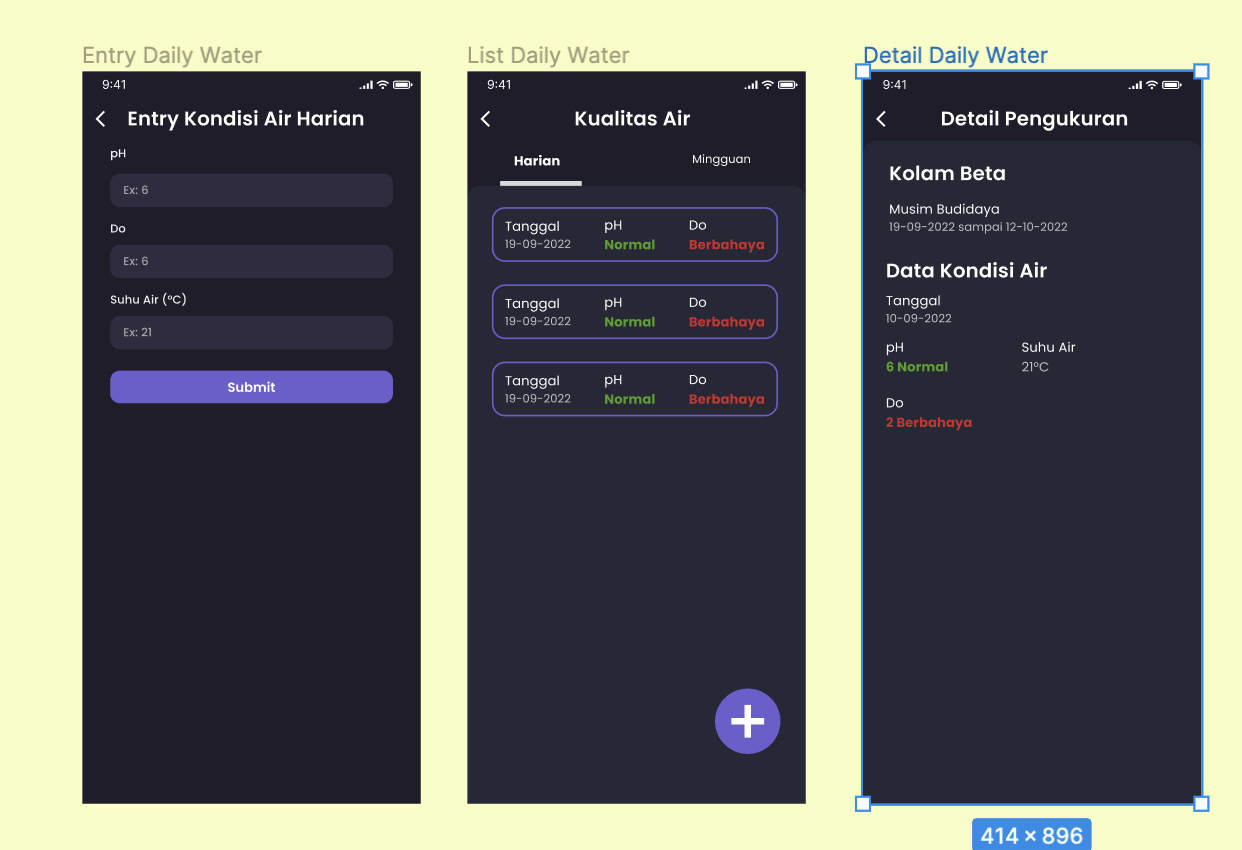
\includegraphics[keepaspectratio, width=6cm]{gambar/mockupairharian}
	\caption{\textit{Mock-up UI Fitur Pencatatan Kualitas Air Harian}}
	\label{gambar:mockupairharian}
	\end{figure}

	\item{\textit{Class Diagram}}
	
	Class Diagram menggambarkan kelas-kelas yang akan dipakai oleh sistem. Umumnya terdapat 3 kelas pada setiap module yaitu class model, controller, dan view. Pada sprint-8 penelitian kali ini penulis membuat 4 class yaitu model yang berwarna biru, view berwarna oranye, controller yang berwarna hijau, dan service yang berwarna kuning.
	 
	 \begin{figure}[H]
	 \centering
	 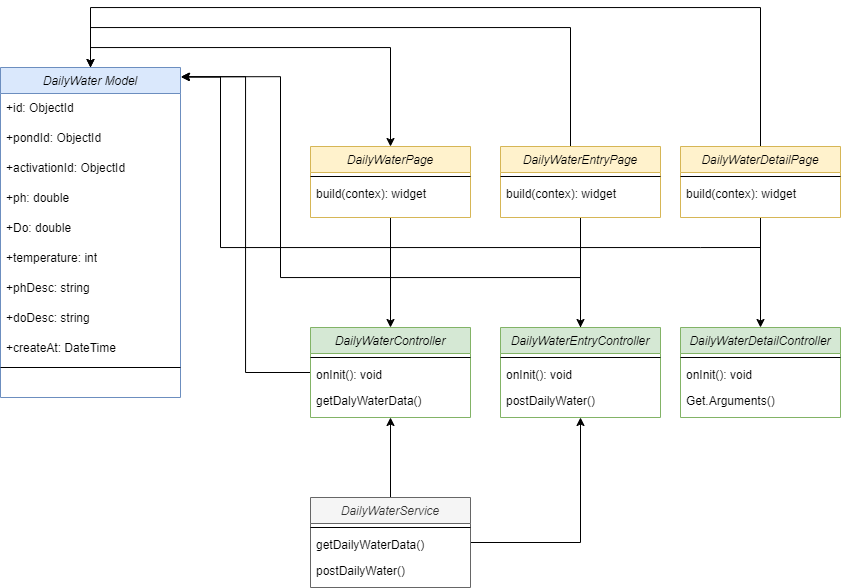
\includegraphics[keepaspectratio, width=6cm]{gambar/dailycd}
	 \caption{\textit{Class Diagram Fitur Sprint-8}}
	 \label{gambar:dailycd}
	 \end{figure}

	\item{\textit{Menerapkan Mockup-UI Fitur Pencatatan Kualitas Air Harian kedalam code flutter}}
	
	Setelah itu, akan dilakukan pengimplementasian \textit{mock-up UI} ke dalam aplikasi menggukan flutter. Pada lampiran 9 terdapat source code dari implementasi fitur pencatatan kualitas air harian yang dikelompokan berdasarkan halaman yang menghasilkan output halaman sebagai seperti dibawah ini.

	\begin{figure}[H]
		\centering
		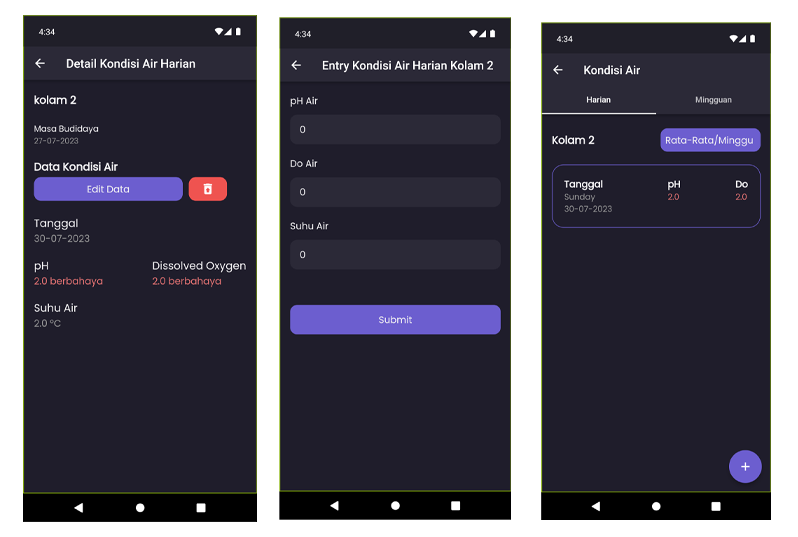
\includegraphics[keepaspectratio, width=8cm]{gambar/sssprint8}
		\caption{\textit{Output dari code pada sprint 8}}
		\label{gambar:sssprint8}
		\end{figure}

	\item{\textit{Mengitegrasikan fitur pencatatan kualitas air harian dengan webservice}}

	Sebelumnya, setiap data pada fitur masih berupa data dummy sehingga perlu diintegrasikan dengan webservice agar aplikasi dapat berjalan dengan data yang asli. Hal yang dilakukan dalam mengintegrasikan fitur pencatatan kualitas air harian dengan webservice terdapat pada lampiran 9.

  \item{Analisis \textit{User Experience}} 
 
  Pada halaman entry daily water quality, pembudidaya harus memasukan data yang diperlukan untuk melakukan daily water quality sesuai dengan kesepakatan saat meeting, seperti pH, Dissolved Oxygen, dan suhu. Selain itu terdapat juga list mengenai data daily water quality yang telah dimasukan yang berisi informasi yang berhubungan dengan daily water quality. Terdapat pula halaman detail daily water quality yang berisi informasi yang lebih detail terkait daily water quality yang telah dilakukan.

\item{Sprint 8 Review dan Sprint 9 Planning}

Sprint 8 diakhiri dengan melakukan weekly meeting pada hari selasa dengan agenda melakukan review dan testing terkait hasil sprint 8 dan melakukan planning untuk sprint 9 dengan rincian:
\begin{enumerate}
	\item{\textit{Review dan Testing hasil dari sprint 8}}

	Telah dilakukan review dan testing oleh penulis selaku developer dengan Scrum Master. Setelah dilakukan testing, Scrum Master menyimpulkan bahwa fitur pencatatan kualitas air harian telah berjalan dengan baik.

	\item{\textit{Sprint Planning untuk Sprint 9}}
	
	Planning untuk sprint 9 yakni membuat fitur pencatatan kualitas air mingguan pada aplikasi \textit{Assistive Aquaculture Breeding Management}.
\end{enumerate}
\end{enumerate}